%%%%%%%%%%%%%%%%%%%%%%%%%%%%%%%%%%%%%%%%%%%%%%%%%%%%%%%%%%%%%%%%%%%%%%%%%%%%%%%%
%% 实验报告模板.tex                                                           %%
%% author: hxp<hxp201406@gmail.com>                                           %%
%% 按照基础物理实验老师发的模板更改形成                                       %%
%%%%%%%%%%%%%%%%%%%%%%%%%%%%%%%%%%%%%%%%%%%%%%%%%%%%%%%%%%%%%%%%%%%%%%%%%%%%%%%%
%% 备注:刚刚的注释刚好是80行,编写代码的时候不要超过80行,就是你的代码不要超 %%
%% 过我注释里面最后面的“%”,超过请换行。                                      %%
%%%%%%%%%%%%%%%%%%%%%%%%%%%%%%%%%%%%%%%%%%%%%%%%%%%%%%%%%%%%%%%%%%%%%%%%%%%%%%%%
%% 模板现在开始,请根据注释把相应的位置更改成对应的内容                       %%
%%%%%%%%%%%%%%%%%%%%%%%%%%%%%%%%%%%%%%%%%%%%%%%%%%%%%%%%%%%%%%%%%%%%%%%%%%%%%%%%


\documentclass{ctexart}


\usepackage{ctex}
\usepackage{amsmath}
\usepackage{amsfonts}
\usepackage{amssymb}
\usepackage{wasysym}
\newcommand{\angstrom}{\text{\normalfont\AA}}  % 定义了原子物理的A
\usepackage{graphicx}
\usepackage{float}
\usepackage{geometry}
\geometry{a4paper,scale=0.8}  % 定义页面大小是A4,缩放是0.8
\usepackage{caption}
\usepackage{subcaption}
\usepackage{enumitem}

\newcommand*{\md}{\mathop{}\!\mathrm{d}}   % 定义微分算子,直立体的d
\newcommand*{\me}{\mathrm{e}}              % 定义自然对数e,同样应当是直立体

% 如果你想要每一段的开头不要空两格,注释掉下面这两行
% \usepackage{parskip}
% \setlength{\parindent}{0cm}

% 默认的\mathbf对希腊字母不生效,这里改下
\usepackage{bm}
\let\Oldmathbf\mathbf
\renewcommand{\mathbf}[1]{\boldsymbol{\Oldmathbf{#1}}}

% 表格默认格内内容和边框没有留出距离,显示分数的时候,分数的上下会贴到边框上
% 因此我增加了表格内容和边框的最短距离是5像素
\usepackage{cellspace}
\setlength{\cellspacetoplimit}{5pt}
\setlength{\cellspacebottomlimit}{5pt}

% \si命令是用来写单位的,单位需要和之前的数字有一个空格的距离,而且应当直立体
% 用法:5 \si{km/h}
\newcommand{\si}[1]{\  \mathrm{#1}}

% 日期不要显示
\date{}

\usepackage{fancyhdr}
\pagestyle{fancy}
\fancyhf{}
\lhead{本文档TeX源代码地址:GitHub源码地址}
\rfoot{第 \thepage 页}
\renewcommand{\headrulewidth}{1pt}
\renewcommand{\footrulewidth}{1pt}

%% 标题三号黑体,作者信息为班级姓名学号
\newcommand{\generatetitle}[6]{\title{\zihao{3}\heiti#1} \author{#2 \quad
    \quad #3 \quad\quad #4 \quad\quad #5 \quad\quad #6} \maketitle\thispagestyle{fancy}}

%% 所有的引言、实验内容与数据处理啥的,用section
\ctexset {
  section = {
    format = \raggedright\zihao{4}\heiti,  % 设置所有section的字号为四号黑体左对齐
    name={,、},                            % 序号后跟顿号
    aftername={\hspace{0pt}},              % 修改序号和标题直接的间距为零
    number=\chinese{section},              % 设置序号为中文
  },
  subsection = {
    format = \raggedright\zihao{5}\heiti,  % 设置所有subsection的字号为五号黑体左对齐
    number={},              % 设置序号为没有序号
  }
}

%% 实验背景、实验目的啥的,用subsection
\ctexset {
  subsection = {
    format = \raggedright\zihao{5}\heiti,  % 所有subsection的字号为五号黑体左对齐
    number={},                             % 设置序号为没有序号
  }
}

%% 把subsection之间加上中括号
\let\oldsubsection\subsection
\renewcommand{\subsection}[1]{\oldsubsection{\!\!\!\!\!\!【#1】}}

%% 摘要和关键词用paragraph

\ctexset {
  paragraph = {
    format = \raggedright\zihao{5}\heiti,  % 所有paragraph的字号为五号黑体左对齐
    number={},                             % 设置序号为没有序号
  }
}

%% 把paragraph之间加上中括号
\let\oldparagraph\paragraph
\renewcommand{\paragraph}[1]{\oldparagraph{#1:\!\!\!\!\!\!}}

%% 再把参考文献的序号去掉
\makeatletter
\renewcommand\@biblabel[1]{}
\makeatother

\begin{document}

\generatetitle{近代物理实验报告——
  材料形貌及光学性质表征}{物理4+4}{胡喜平}{U201811966}{hxp201406@gmail.com}{https://hxp.plus/}

\paragraph{摘要}
本次实验主要练习原子力显微镜和可见分光光度计的使用,并用这两个仪器测量材料的表面
形貌和禁带宽度。

% 关键词
\paragraph{关键词}
原子力显微镜、禁带宽度、半导体、材料形貌的测量

\section{引言}
\subsection{实验背景}
原子力显微镜是一种利用分子间相互作用的引力或者斥力来对材料表面形态进行扫描的一种
显微镜,它的分辨率在纳米量级,在材料科学上有广泛应用。而禁带宽度是半导体材料的一
个重要性质,用来表示价键束缚的强弱,通常用光谱法进行测量。本次实验练习使用原子力
显微镜和可见分光光度计测量材料的表面形貌和半导体的禁带宽度。

\subsection{实验目的}
学会安装原子力显微镜的探针,调节显微镜的激光,之后用原子力显微镜扫描不同材料的表
面样貌。学会可见分光光度计的使用,用实验仪器的数据来计算材料的禁带宽度。

\section{实验内容与数据处理}
\subsection{实验原理}
原子力显微镜是一种利用范德瓦尔斯力来探测样品表面形貌的仪器,装置的示意图如图(a
)所示,微悬臂上的探针距离待测表面很近,待测表面的原子和探针上的原子之间有引力或
者斥力,使得微悬臂微小形变。激光打在微悬臂上反射,使得微悬臂的微小变化造成反射激
光角度变化,进而测量探针和原子之间的距离。

\begin{figure}[htbp]
  \centering
  \begin{subfigure}{.25\textwidth}
    \centering
    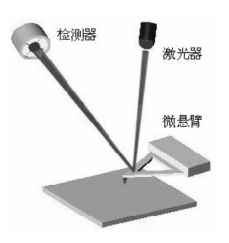
\includegraphics[width=\linewidth]{figures/AFM}
    \caption{AFM测量原理示意简图}
  \end{subfigure}
  \begin{subfigure}{.35\textwidth}
    \centering
    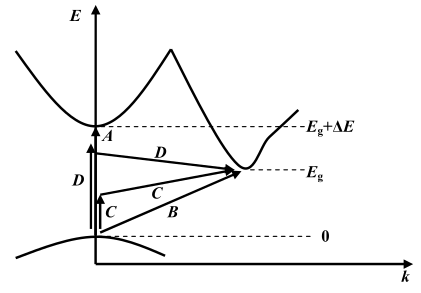
\includegraphics[width=\linewidth]{figures/禁戒的代间直接跃迁}
    \caption{价电子的代间跃迁}
  \end{subfigure}
    \begin{subfigure}{.35\textwidth}
    \centering
    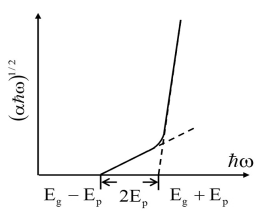
\includegraphics[width=\linewidth]{figures/间接跃迁情况下吸收系数}
    \caption{价电子间接跃迁光学禁带宽度的计算}
  \end{subfigure}
\end{figure}

半导体吸收光子会发生越迁,其中越迁有直接越迁和间接越迁两种形式。图(b)中,入射
光子能量大于$E_g + \Delta E$时,发生像箭头A那样的直接跃迁。能量介于$E_g$到
$E_g + \Delta E$之间时,发生像箭头B那样的间接跃迁。

其中间接跃迁大致分为两种情况,C过程是吸收声子的,D过程是放出声子的。声子的能量是
$E_p$,则C过程光子能量$E_g - E_p$,D过程光子能量$E_g + E_p$。

对于间接跃迁,光子的吸收系数$\alpha$与入射光子能量有平方关系,因此我们做图(c)
可以求出光学禁带宽度$E_g$。

实验中能从仪器上获得的数据是透射率$T$,应当用$T$计算吸光度$A$,即

\begin{equation*}
  \begin{aligned}
    A = \lg \dfrac{1}{T} 
  \end{aligned}
\end{equation*}

之后运用朗伯-比尔定律,即$A$正比与$\alpha$。

\subsection{实验内容}
为原子力显微镜安装探针,调整激光使激光照射在检测器的中央,放入样品,用电脑控制原
子力显微镜对样品表面进行扫描,每次扫描得到不同的图像。

使用可见分光光度计,放入镀膜后的玻璃片和没有镀膜的玻璃片,对样品进行扫描,得到不
同波长下的透射率。

从可见分光光度计上拷贝不同波长下的透射率数据,之后进行实验数据的处理,得到样品上
镀膜材料的禁带宽度。

\subsection{实验结果的分析和结论}

在调整好探针和光路以后,首先扫描了光栅,刚开开始选择扫描范围为5000nm,后来发现没
有扫描出几个周期,决定扩大扫描范围为12000nm。最终得到横向力的图像为

\begin{figure}[H]
  \centering
  \begin{subfigure}{.49\textwidth}
    \centering
    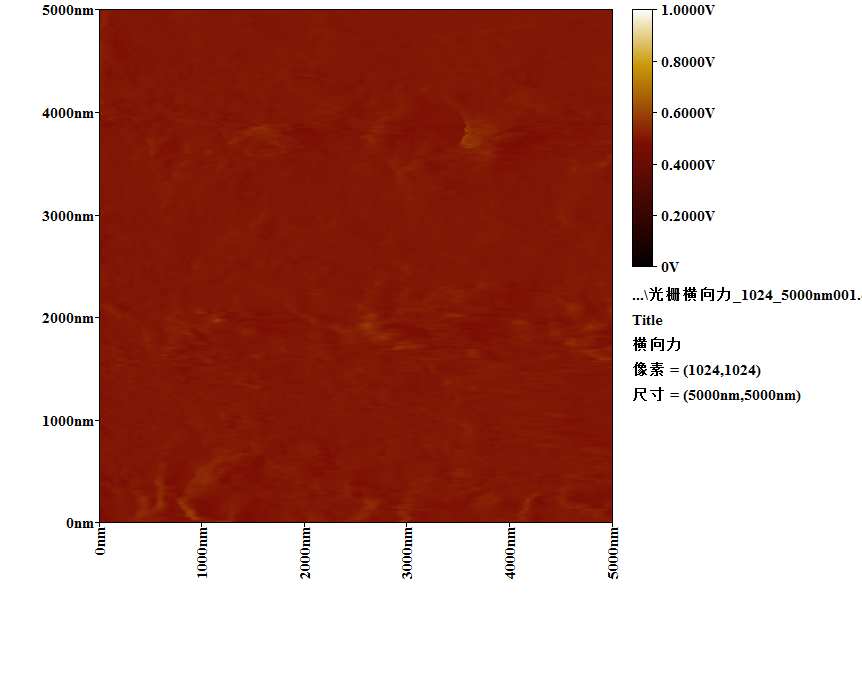
\includegraphics[width=\linewidth]{AFM结果图像/光栅横向力_1024_5000nm}
    \caption{光栅横向力扫描结果,横向力,二维,分辨率1024,扫描范围5000nm}
  \end{subfigure}
  \begin{subfigure}{.49\textwidth}
    \centering
    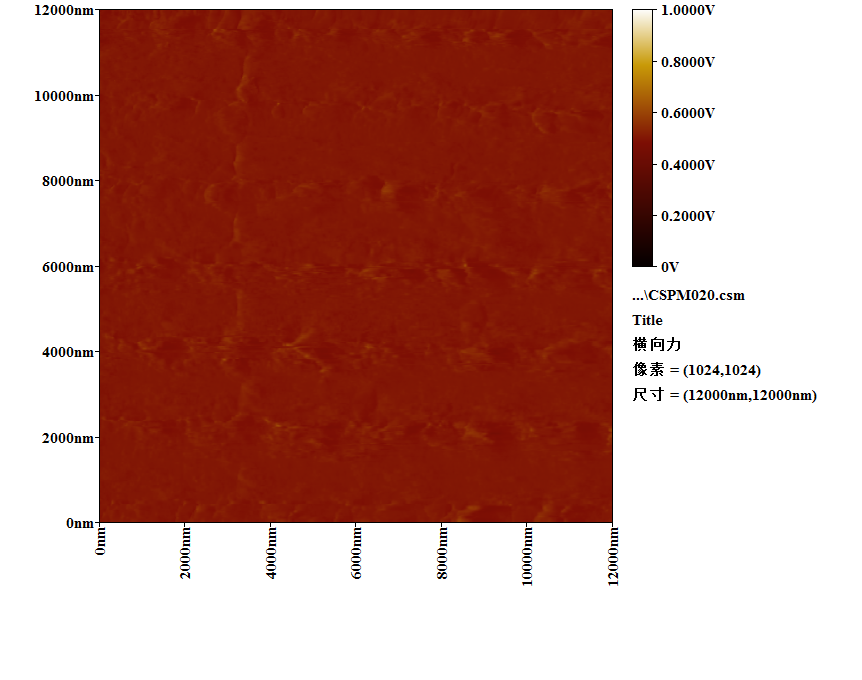
\includegraphics[width=\linewidth]{AFM结果图像/光栅横向力_1024_12000nm}
    \caption{光栅横向力扫描结果,横向力,二维,分辨率1024,扫描范围12000nm}
  \end{subfigure}
\end{figure}

横向力三维图像为

\begin{figure}[H]
  \centering
  \begin{subfigure}{.49\textwidth}
    \centering
    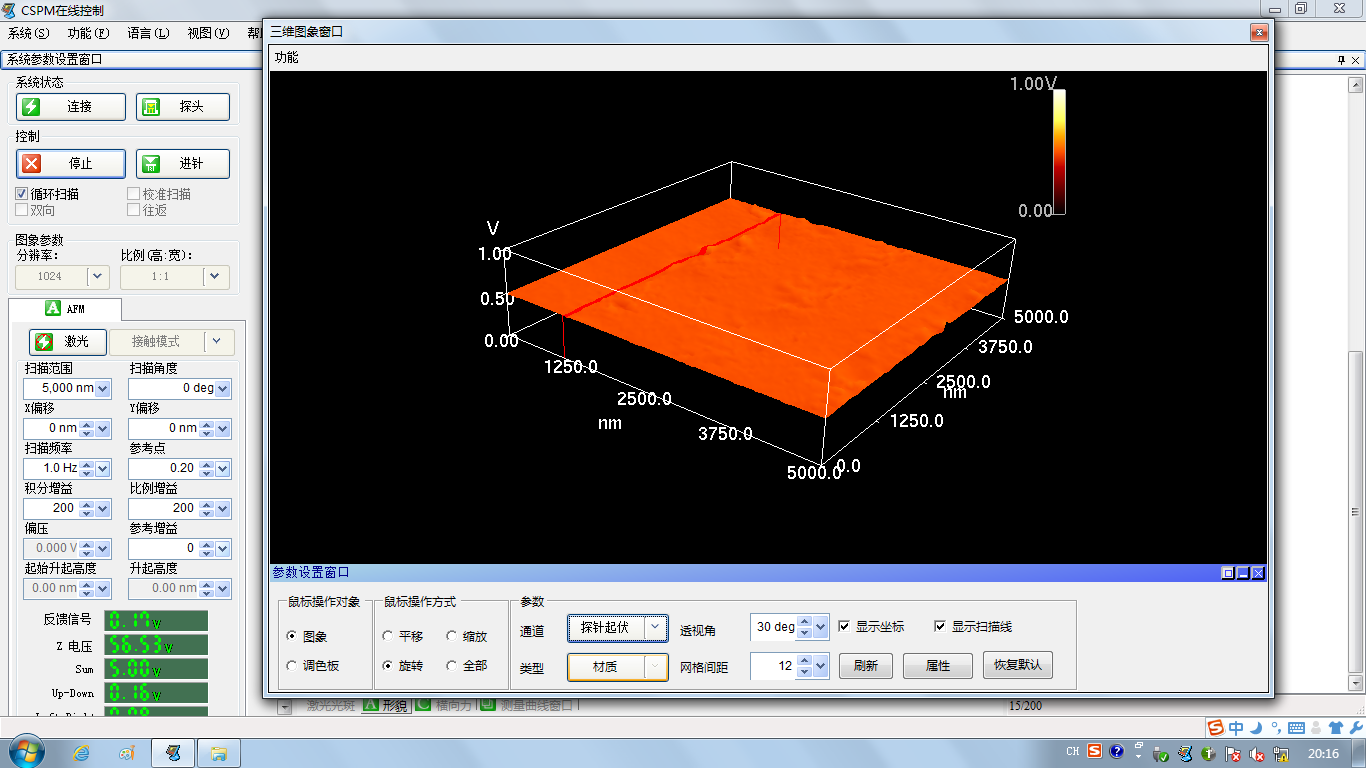
\includegraphics[width=\linewidth]{AFM结果图像/光栅横向力三维_1024_5000nm}
    \caption{光栅横向力扫描结果,横向力,三维,分辨率1024,扫描范围5000nm}
  \end{subfigure}
  \begin{subfigure}{.49\textwidth}
    \centering
    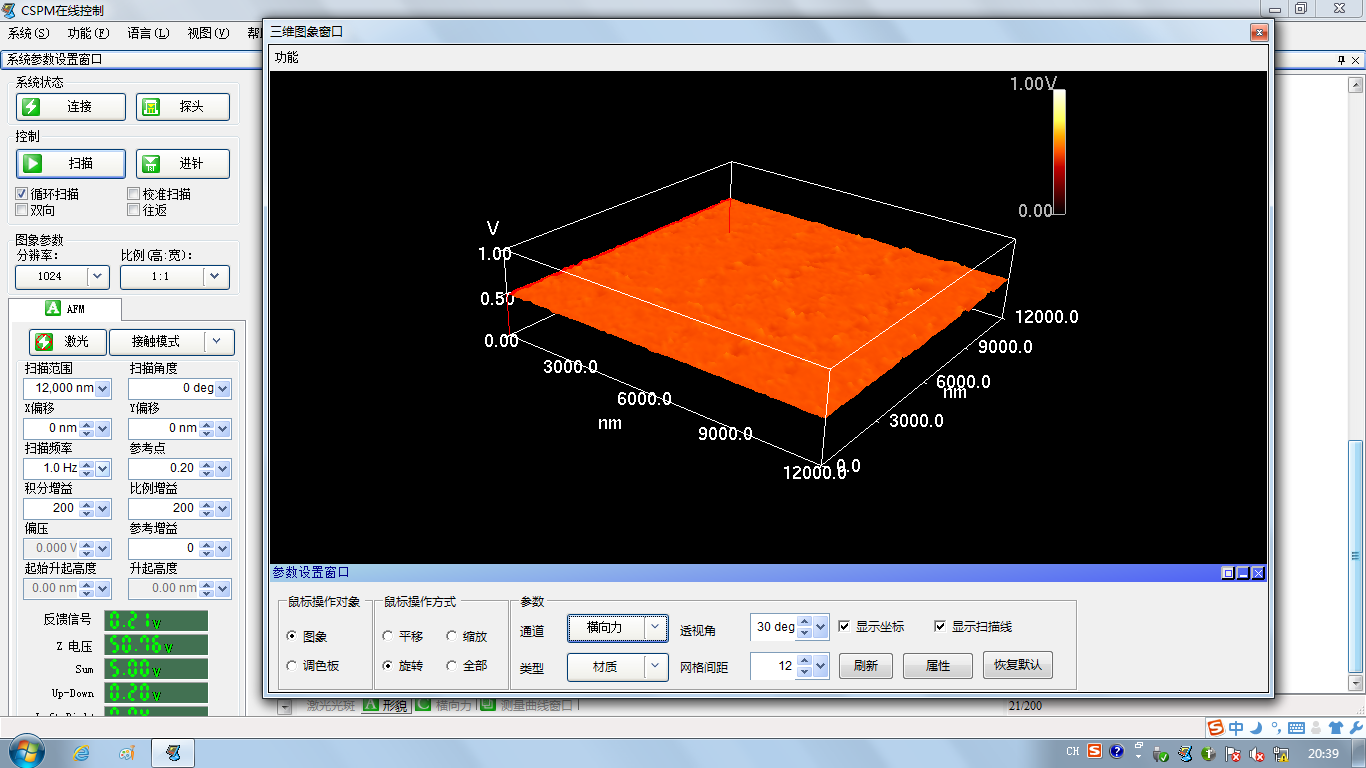
\includegraphics[width=\linewidth]{AFM结果图像/光栅横向力三维_1024_12000nm}
    \caption{光栅横向力扫描结果,横向力,三维,分辨率1024,扫描范围12000nm}
  \end{subfigure}
\end{figure}

光栅表面样貌的图像为

\begin{figure}[H]
  \centering
  \begin{subfigure}{.49\textwidth}
    \centering
    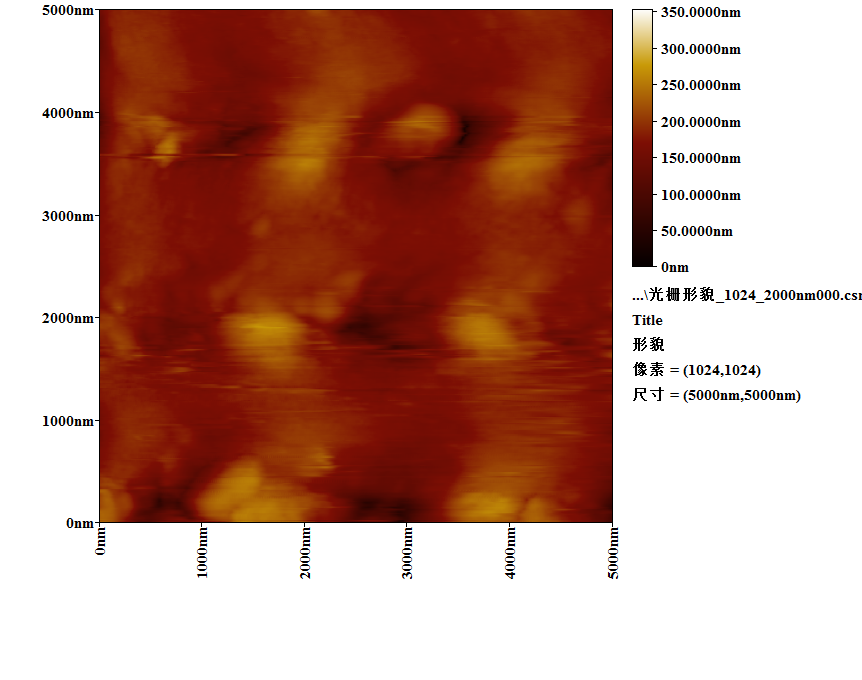
\includegraphics[width=\linewidth]{AFM结果图像/光栅表面样貌_1024_5000nm}
    \caption{光栅横向力扫描结果,表面样貌,二维,分辨率1024,扫描范围5000nm}
  \end{subfigure}
  \begin{subfigure}{.49\textwidth}
    \centering
    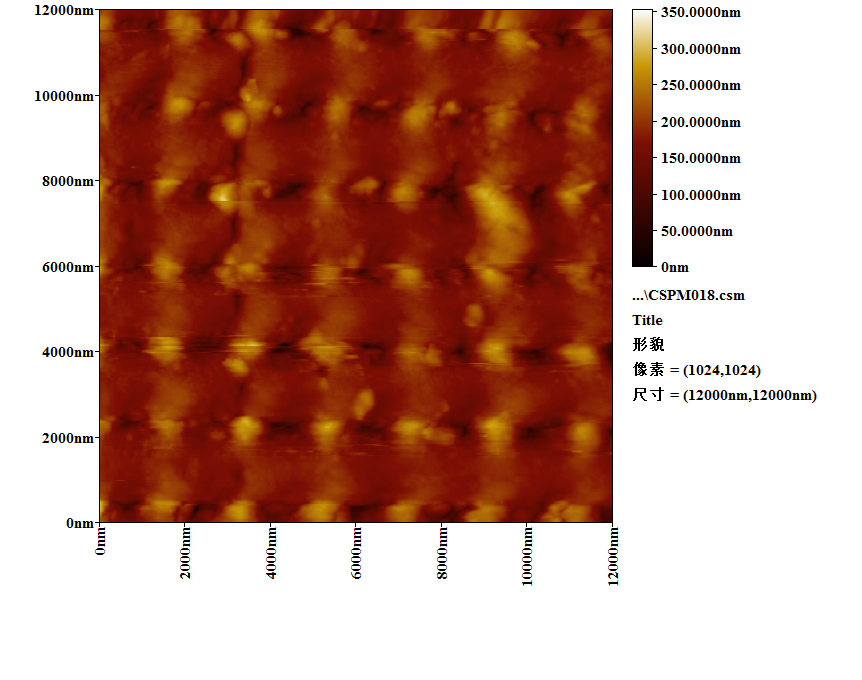
\includegraphics[width=\linewidth]{AFM结果图像/光栅表面样貌_1024_12000nm}
    \caption{光栅横向力扫描结果,表面样貌,二维,分辨率1024,扫描范围12000nm}
  \end{subfigure}
\end{figure}

表面样貌三维图像为

\begin{figure}[H]
  \centering
  \begin{subfigure}{.49\textwidth}
    \centering
    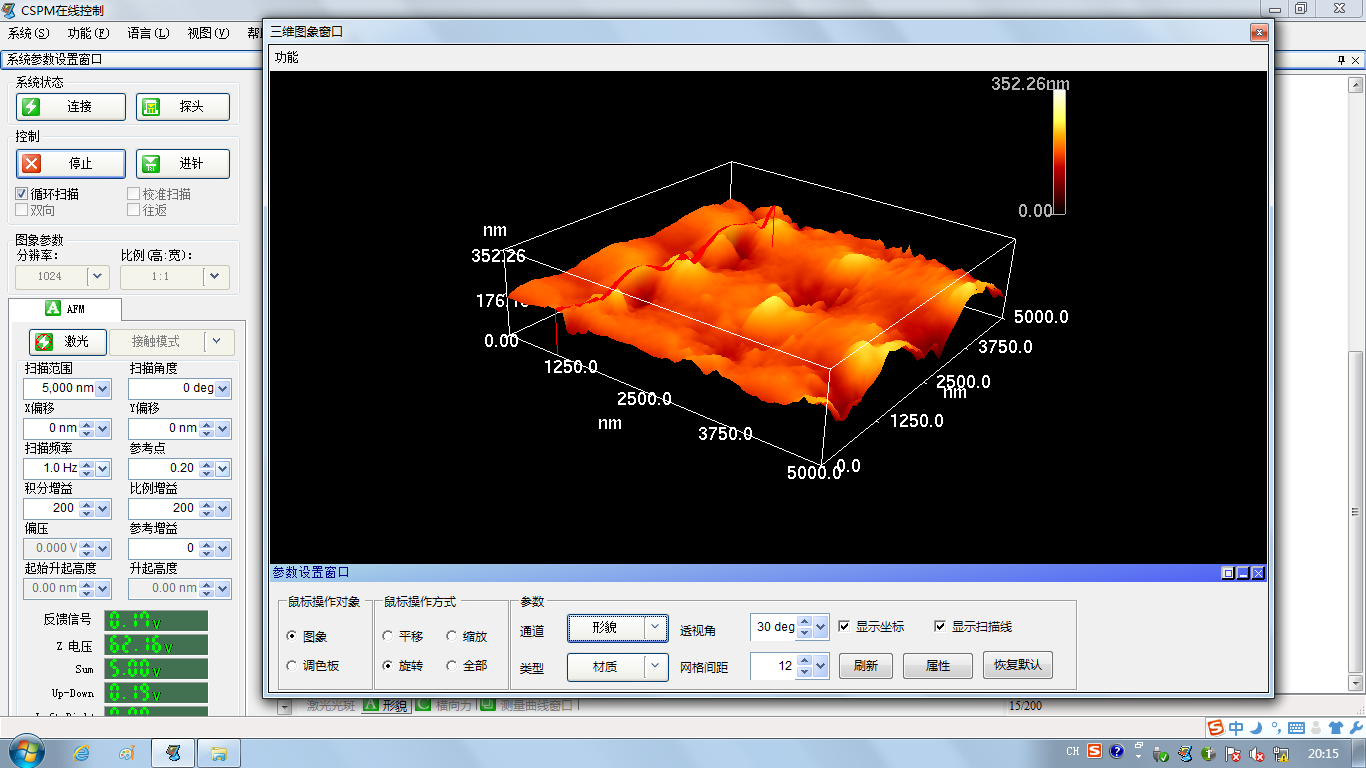
\includegraphics[width=\linewidth]{AFM结果图像/光栅表面样貌三维_1024_5000nm}
    \caption{光栅横向力扫描结果,表面样貌,三维,分辨率1024,扫描范围5000nm}
  \end{subfigure}
  \begin{subfigure}{.49\textwidth}
    \centering
    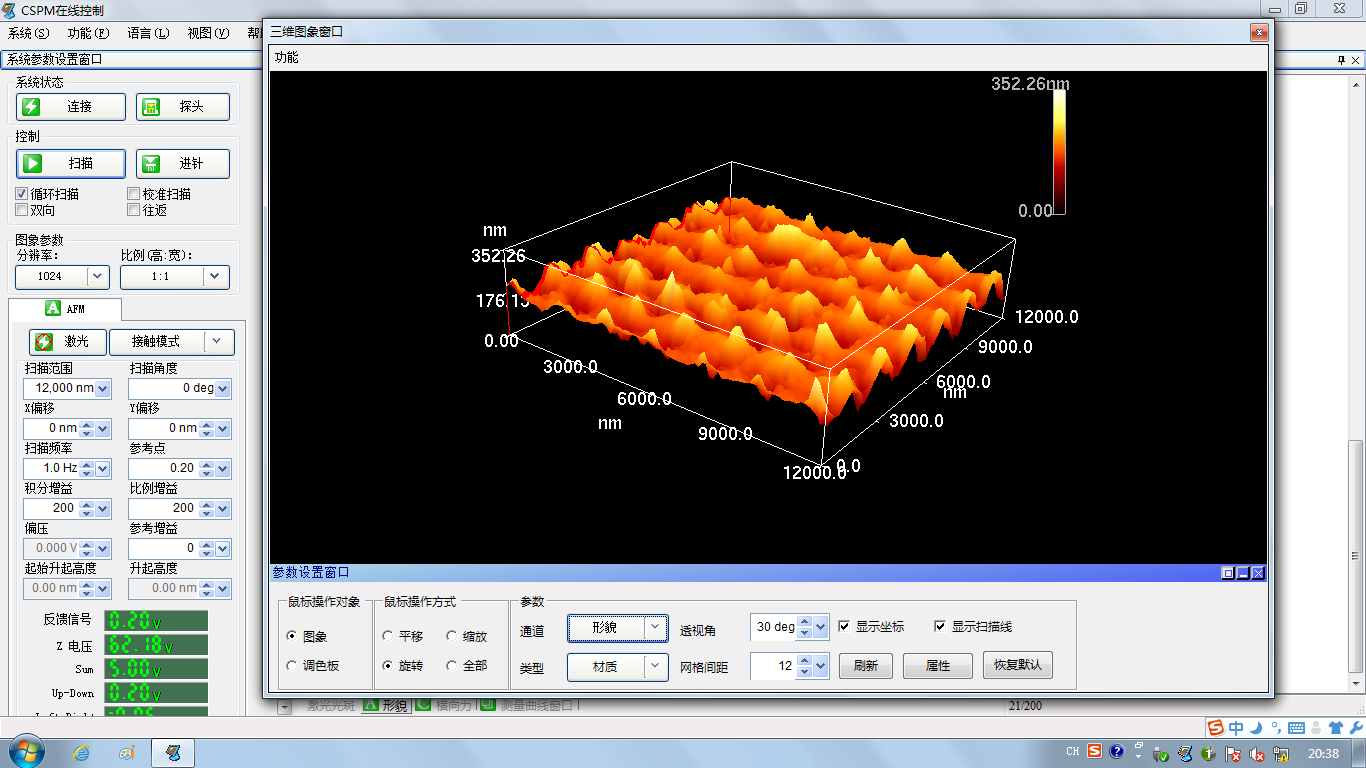
\includegraphics[width=\linewidth]{AFM结果图像/光栅表面样貌三维_1024_12000nm}
    \caption{光栅横向力扫描结果,表面样貌,三维,分辨率1024,扫描范围12000nm}
  \end{subfigure}
\end{figure}

从图像中看出光栅的周期大致为2000nm。之后对光盘扫描,使用不同分辨率

\begin{figure}[H]
  \centering
  \begin{subfigure}{.49\textwidth}
    \centering
    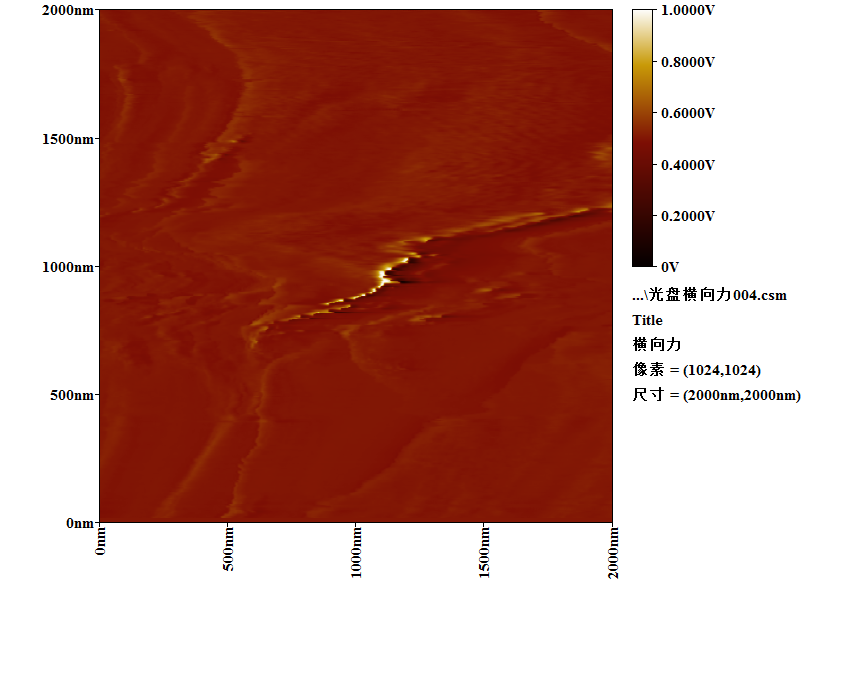
\includegraphics[width=\linewidth]{AFM结果图像/光盘横向力_1024_2000nm}
    \caption{光盘横向力扫描结果,横向力,二维,分辨率1024,扫描范围2000nm}
  \end{subfigure}
  \begin{subfigure}{.49\textwidth}
    \centering
    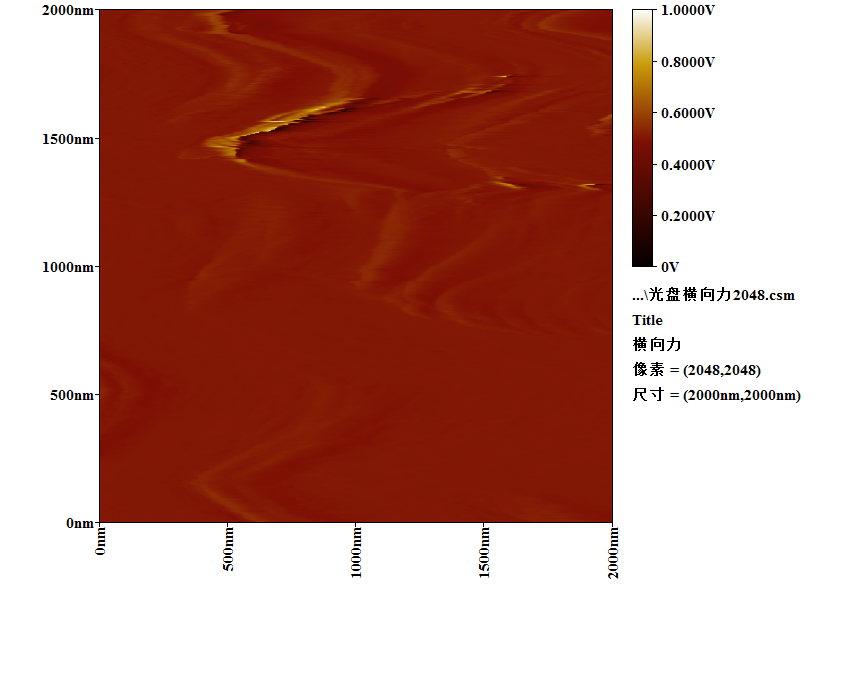
\includegraphics[width=\linewidth]{AFM结果图像/光盘横向力_2048_2000nm}
    \caption{光盘横向力扫描结果,横向力,二维,分辨率2048,扫描范围2000nm}
  \end{subfigure}
\end{figure}

\begin{figure}[H]
  \centering
  \begin{subfigure}{.49\textwidth}
    \centering
    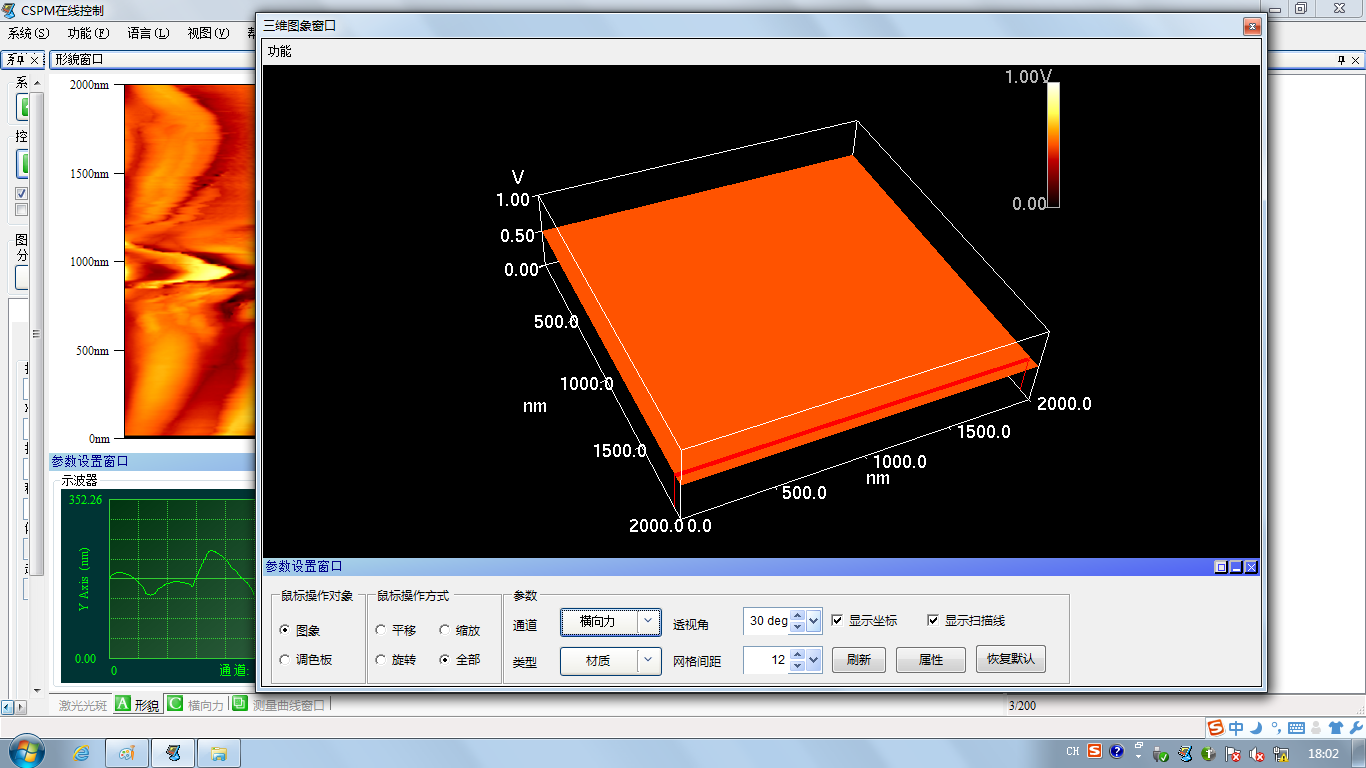
\includegraphics[width=\linewidth]{AFM结果图像/光盘横向力三维_1024_2000nm}
    \caption{光盘横向力扫描结果,表面样貌,三维,分辨率1024,扫描范围2000nm}
  \end{subfigure}
  \begin{subfigure}{.49\textwidth}
    \centering
    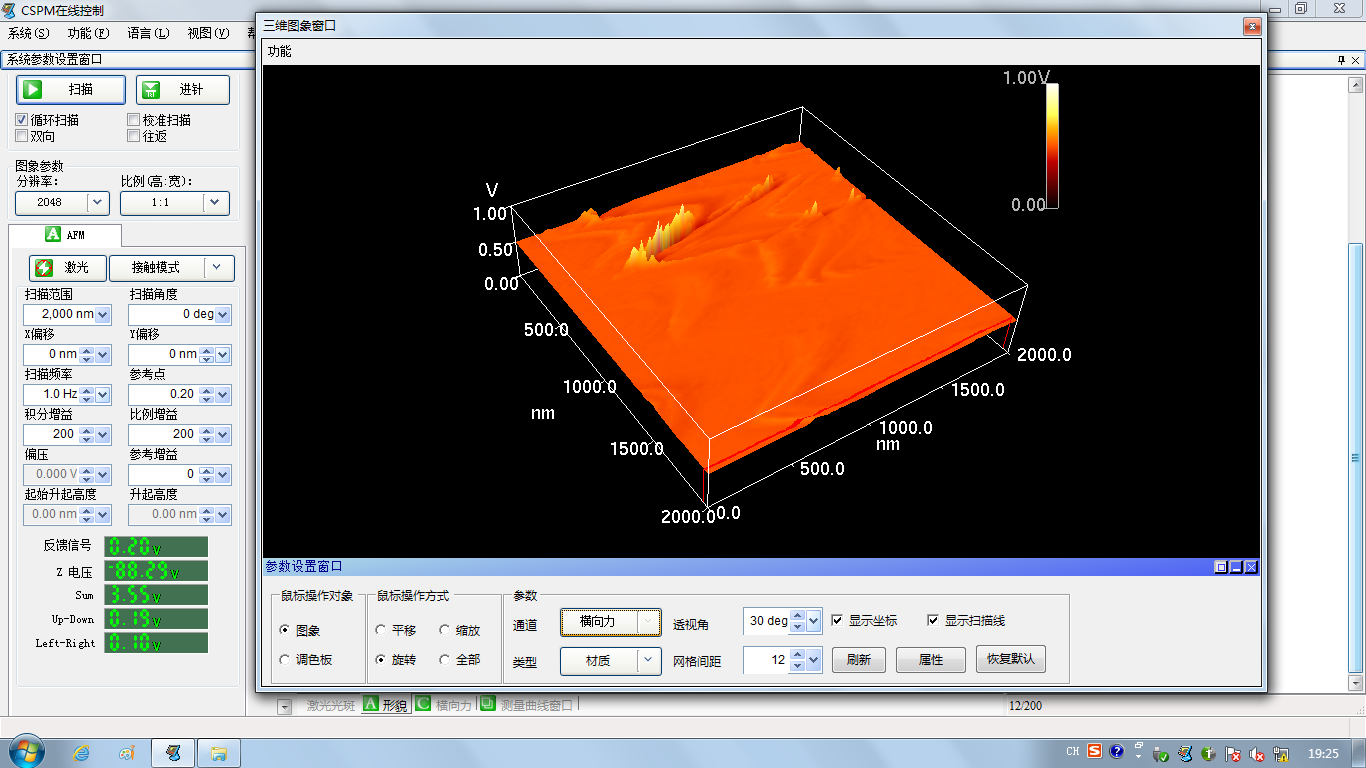
\includegraphics[width=\linewidth]{AFM结果图像/光盘横向力三维_2048_2000nm}
    \caption{光盘横向力扫描结果,表面样貌,三维,分辨率2048,扫描范围2000nm}
  \end{subfigure}
\end{figure}

\begin{figure}[H]
  \centering
  \begin{subfigure}{.49\textwidth}
    \centering
    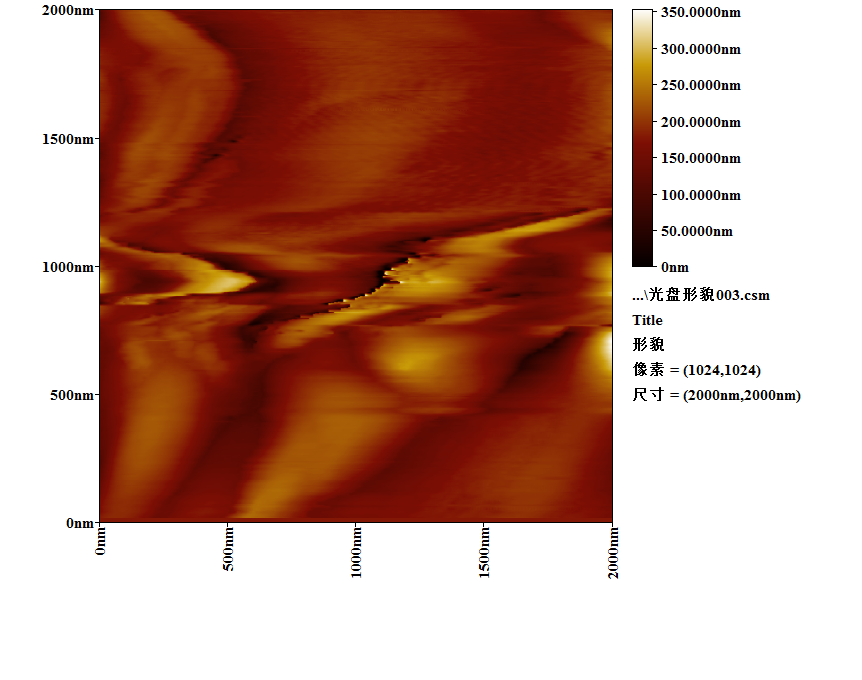
\includegraphics[width=\linewidth]{AFM结果图像/光盘表面样貌_1024_2000nm}
    \caption{光盘表面样貌扫描结果,表面样貌,二维,分辨率1024,扫描范围2000nm}
  \end{subfigure}
  \begin{subfigure}{.49\textwidth}
    \centering
    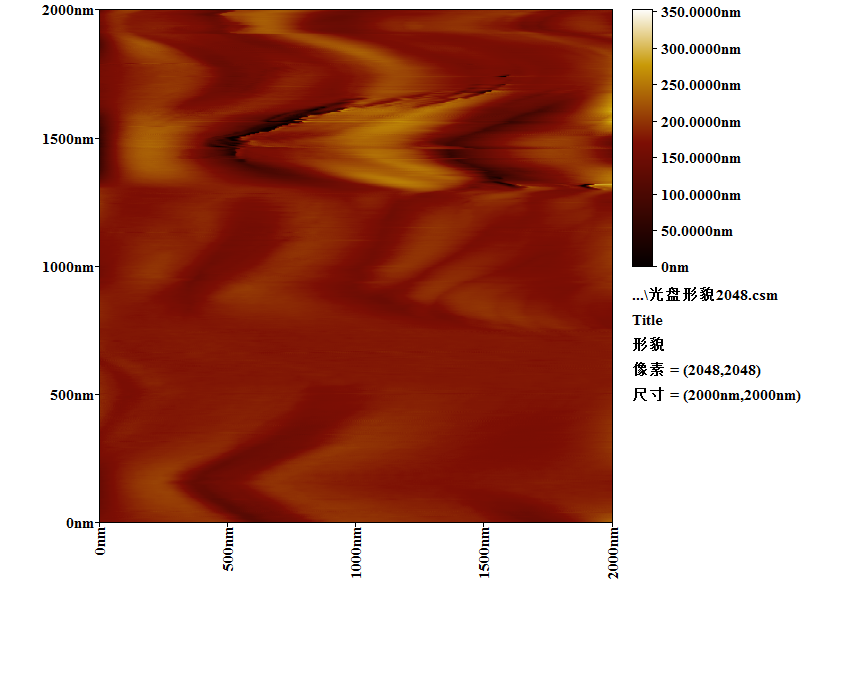
\includegraphics[width=\linewidth]{AFM结果图像/光盘表面样貌_2048_2000nm}
    \caption{光盘表面样貌扫描结果,表面样貌,二维,分辨率2048,扫描范围2000nm}
  \end{subfigure}
\end{figure}

\begin{figure}[H]
  \centering
  \begin{subfigure}{.49\textwidth}
    \centering
    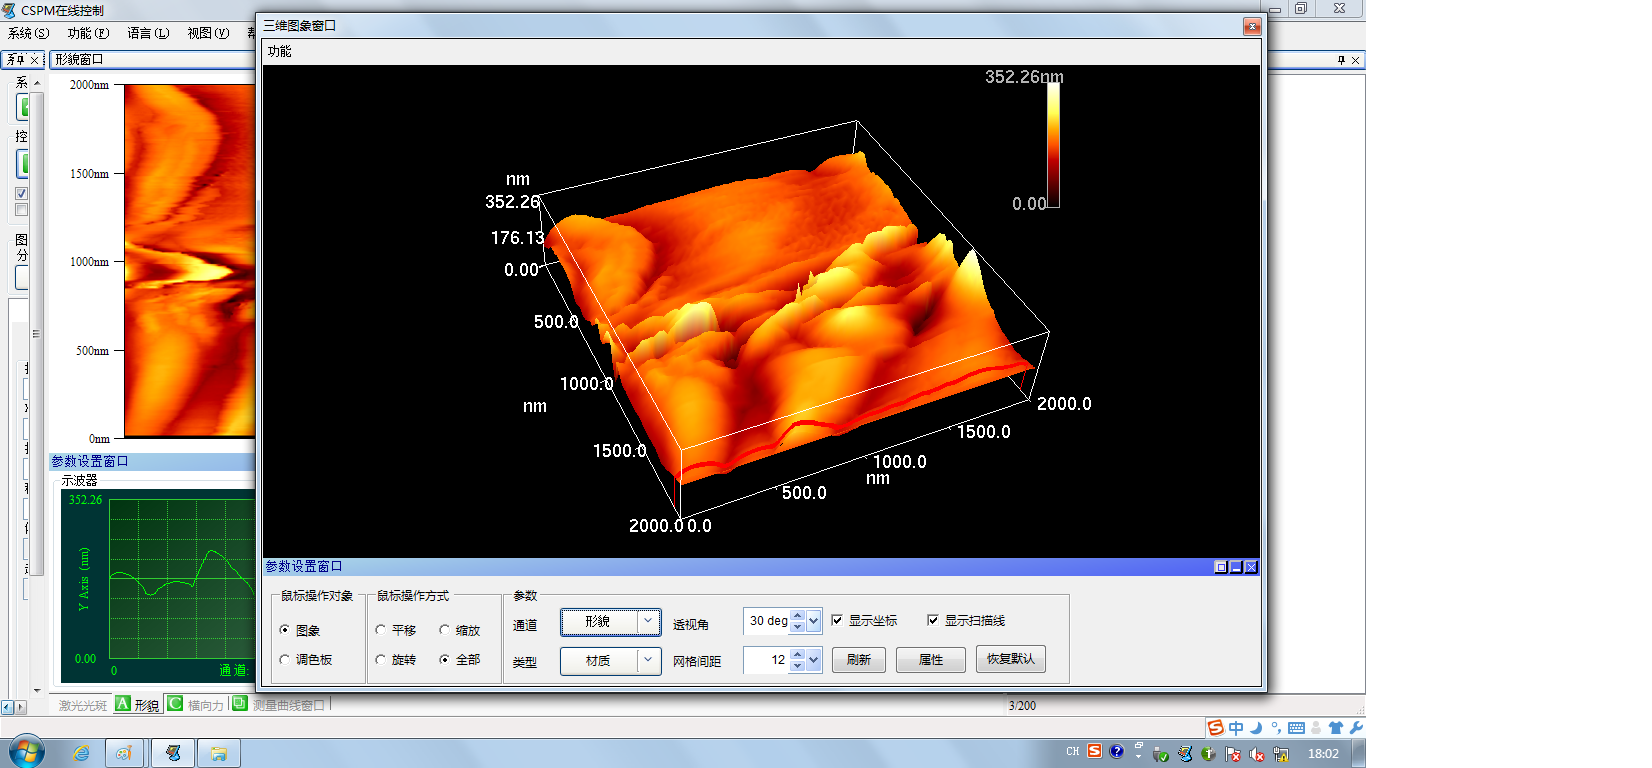
\includegraphics[width=\linewidth]{AFM结果图像/光盘表面样貌三维_1024_2000nm}
    \caption{光盘表面样貌扫描结果,表面样貌,三维,分辨率1024,扫描范围2000nm}
  \end{subfigure}
  \begin{subfigure}{.49\textwidth}
    \centering
    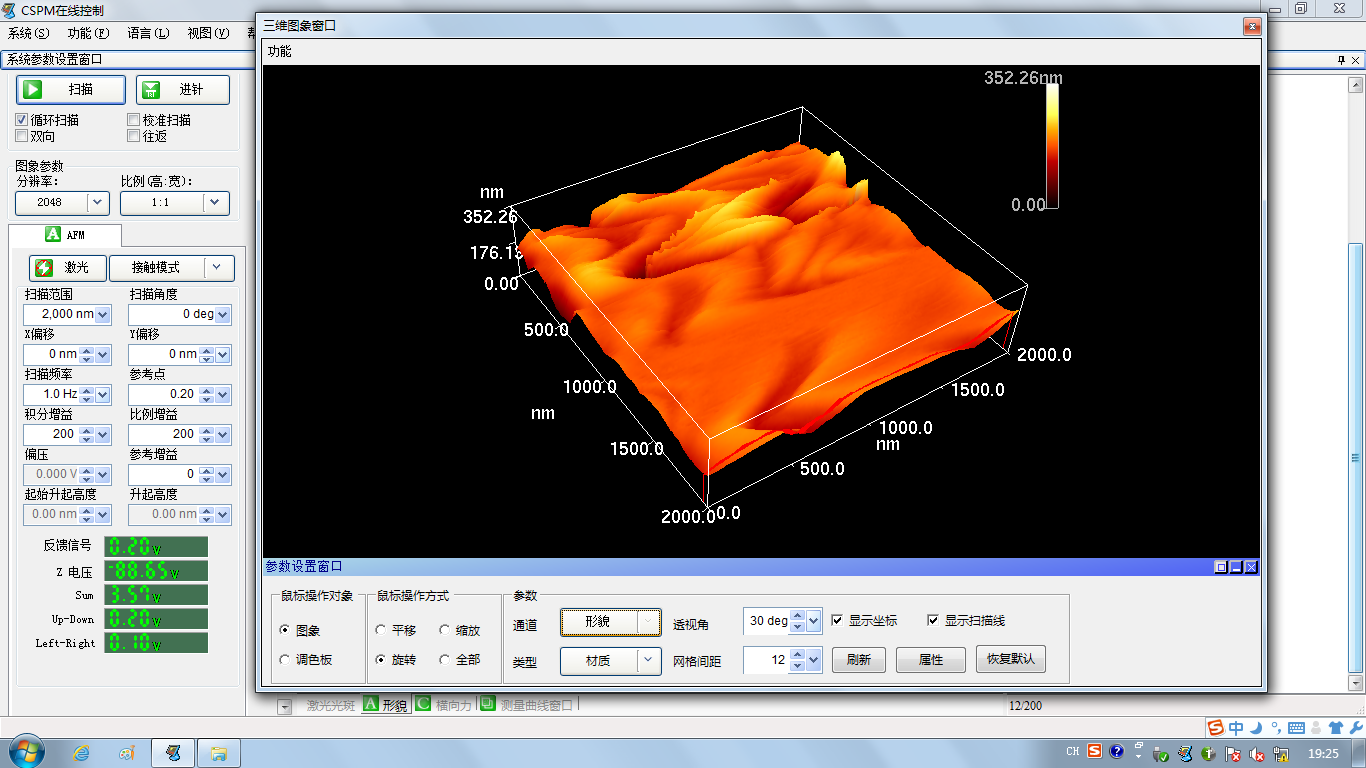
\includegraphics[width=\linewidth]{AFM结果图像/光盘表面样貌三维_2048_2000nm}
    \caption{光盘表面样貌扫描结果,表面样貌,三维,分辨率2048,扫描范围2000nm}
  \end{subfigure}
\end{figure}

之后是禁带宽度的测量,这个实验的难度主要是对数据的分析与处理。首先我们求的应当是
膜的透光率,因此最开始只放玻璃片进行扫描,这就是镀膜0分钟的数据。之后扫描的是玻
璃镀膜的数据,不是膜的透过率,而是膜和玻璃透过率的乘积。

具体实验的处理程序连同代码在附件,我也上传了一个在GitHub,地址为:
https://github.com/hxp-plus/band-gap-fitting

这是项目的目录

\begin{figure}[H]
  \centering
  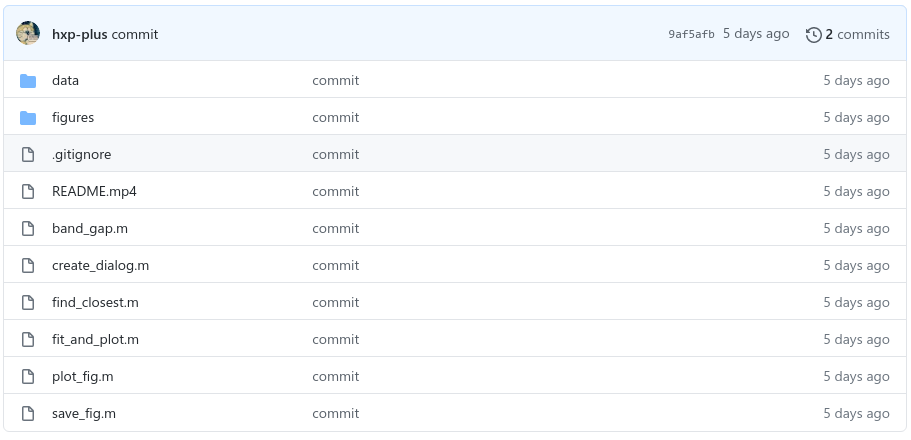
\includegraphics[width=\linewidth]{figures/禁带宽度数据处理程序}
  \caption{禁带宽度数据处理程序项目目录}
\end{figure}

其中数据以mat文件格式保存在data目录下,程序运行的时候输出的图像都保存在figures目
录下。程序会在figures目录下创建相应的文件夹,表明图像是什么,然后在创建的文件夹
里面将画出的图像保存为fig绘图原始数据、eps矢量图、png位图三种格式。

程序首先会绘制并保存原始图像,之后绘制求禁带宽度需要的图像,之后弹窗让用户选择
范围对图像进行缩放,并绘制保存缩放的图像,最后会弹窗两次让用户选择线性拟合的范围
,并绘制线性拟合后的图像。

具体程序的用法,我录制了一个视频README.mp4,可以参考

这个程序输出了下面四个图像:


\subsection{实验中遇到的问题及解决方法}



\section{实验小结}
\subsection{体会或收获}
\subsection{实验建议}
内容
\section{参考文献}
\begin{itemize}[leftmargin=0pt]
  \item[] 作者,题目,期刊名或书名,页码,出版时间
  \item[] 其他作者,题目,期刊名或书名,页码,出版时间
\end{itemize}
\end{document} 
